\section{Prototypage}
\subsection{Implémentation}
\begin{frame}
 \frametitle{Prototypage}
 Un réseau de capteurs sans fil a été déployé dans une maison pendant 12 jours dans un contexte de gestion d'énergie.
 L'implémentation de leur prototype ne requiert que 15,8k, parseur XML, serveur HTTP et file TCP/IP inclus !
 \begin{figure}
  \centering
  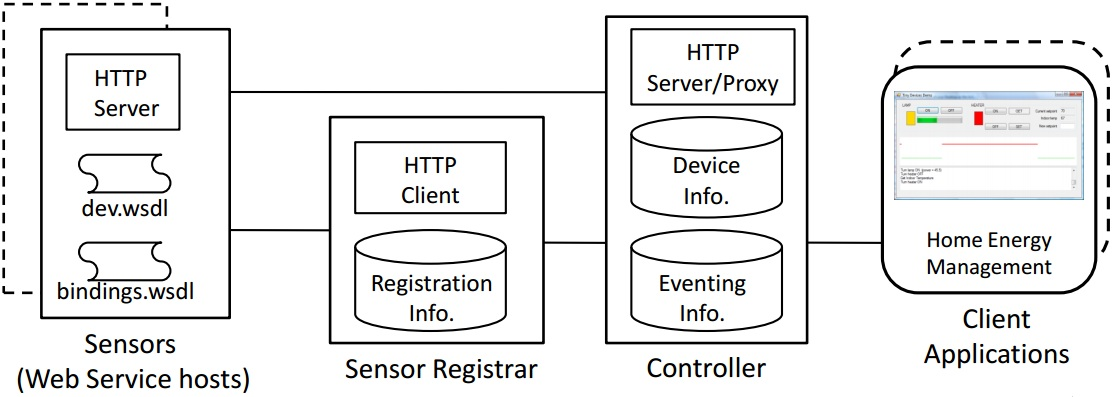
\includegraphics[scale=0.36]{figures/implementation.jpg}
  \caption{Diagramme d'implémentation du service web}
 \end{figure} 
\end{frame}

\begin{frame}
 \frametitle{Implémentation}
 \framesubtitle{Capteurs}
 Chaque capteur contient deux fichiers WSDL:
 \begin{enumerate}
  \item \textbf{\texttt{dev.wsdl}} Décrit complètement les méthodes supportées par le capteur et accessibles pour l'utilisateur. Noms de méthodes avec leurs paramètres, type des paramètres et de la valeur retournée.
  \item \textbf{\texttt{bindigs.wsdl}} Importe \texttt{dev.wsdl} et ajoute 3 méthodes accessibles seulement pour le controleur:
   \begin{enumerate}
    \item \texttt{void eventOn(string eventName)}
    \item \texttt{void eventOff(string eventName)}
    \item \texttt{void setHandlerURL(string url)}
   \end{enumerate}
   Pour autoriser à poster l'évenement \texttt{eventName} à l'adresse URL \texttt{url}
 \end{enumerate}
 Le capteur lance un serveur HTTP qui accède au fichier \texttt{bindigs.wsd}.\\
 La requête est encodée dans l'URL et retourne un fichier XML.
\end{frame}

\begin{frame}
 \frametitle{Implémentation}
 pour ajouter un nouveau capteur dans le réseau, l'\textit{enregistreur} (Sensor Registrar) télécharge les fichiers wsdl et enregistres les données dans un fichier XML avec une IP préétablie et un nom donné par l'utilisateur.
 Ensuite il envoie le XML au controleur.
 Il peut être implémenté aussi bien dans un PC qu'un point d'accès 802.15.4.\\
 \vspace{4mm}
 Le \textit{controleur} agit comme un serveur HTTP.\\
 \texttt{http://Controller/index.htm} retourne la liste des capteurs enregistrés.\\
 \texttt{http://Controller/wsdl/<sensorName>.wsdl} retourne la description WSDL du capteur \texttt{<sensorName>}
\end{frame}


\newcommand{\unite}{(octets)}
\begin{frame}%[fragile]
 \frametitle{Implémentation}
 \framesubtitle{Mémoire utilisée}
 \begin{center}
 \begin{tabular}{|l|r|r|r|}
  \hline
  Module & Code & Data & Const\footnote{\textbf{Const}: Constantes enregistrées dans la ROM}\\
  ~ & \unite & \unite & \unite \\
  \hline
  Librairies & 804 & 2 & 76\\
  controle hardware & 408 & 78 & 12\\
  Driver radio & 4282 & 404 & 14\\
  TCP/IP & 2964 & 332 & 4\\
  Serveur web+parseur XML & 2380 & 54 & 4864\\
  \hline
  \textbf{Total} & \textbf{10838} & \textbf{870} & \textbf{4970}\\
  \hline
 \end{tabular}
 \end{center}
\end{frame}

\subsection{Déploiement}
\begin{frame}
 \frametitle{Déploiement}
 Le réseau de capteurs déployé contient aussi des capteurs communément utilisés pour la sécurité.
 Par exemple, ils ont utilisés des capteurs de mouvement, d'ouverture de porte, ...
 Mais ils ont également placé des capteurs permettant de mesurer et regler la consomation d'énergie de n'importe quel appareil grâce à leurs \textit{smart-sockets}.
\end{frame}

\newcommand{\smartsocket}{\textit{smart-socket}~}
\begin{frame}
 \frametitle{Diagramme du \smartsocket}
 \begin{figure}
  \centering
  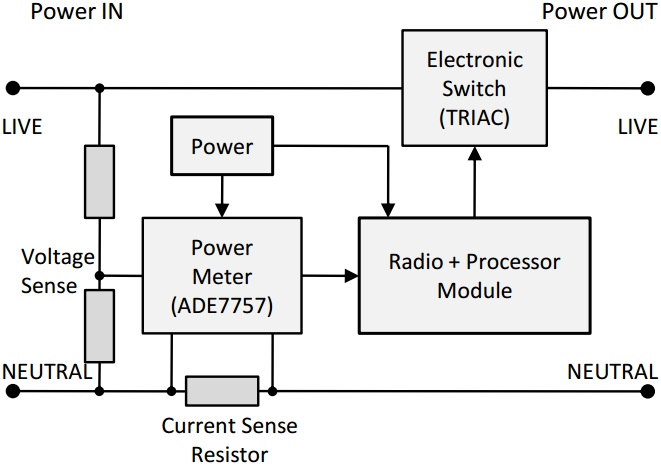
\includegraphics[scale=0.35]{figures/smartsocket.jpg}
  \caption{Le \smartsocket}
 \end{figure} 
 À brancher au réseau électrique, le \smartsocket permet de mesurer l'énergie électrique consommée par l'appareil branché au \smartsocket et de l'éteindre ou l'allumer à distance.
 Il supporte jusqu'à 2kW\\
 %On a besoin de visualiser la consomation d'énergie de chaque appareil.
 %Combiné avec des capteurs d'ouverture de porte et capteur de mouvements, un algorithme de gestion d'énergie peut être appliqué.
 %Lors de l'expérience, des smart-sockets ont été utilisés pour les lampes et appareils de divertissement utilisés la plupart du temps.
\end{frame}

\def \exsca {0.21}
\begin{frame}
 \frametitle{Quelques données collectées\footnote{L'unité de l'axe du temps n'est pas affiché pour protéger la vie privée des résidents.}}
 \begin{figure}
  \begin{minipage}[c]{.46\linewidth}
   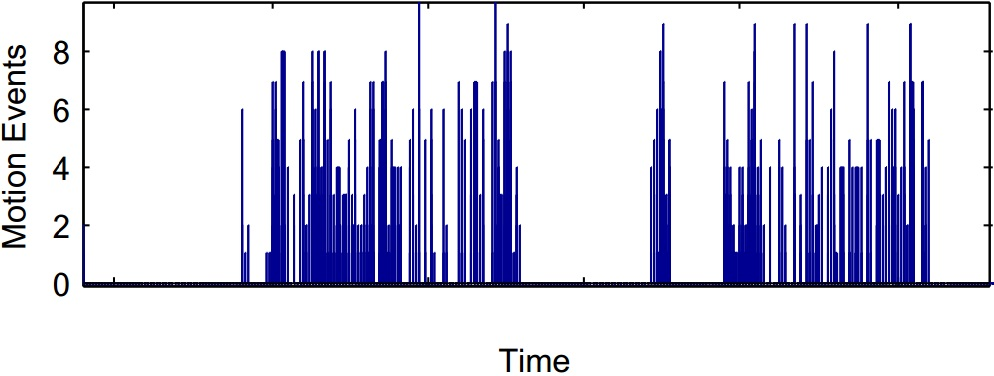
\includegraphics[scale=\exsca]{figures/EXmovement.jpg}
   \caption{Détecteur de mouvements}
  \end{minipage}
  \begin{minipage}[c]{.46\linewidth}
   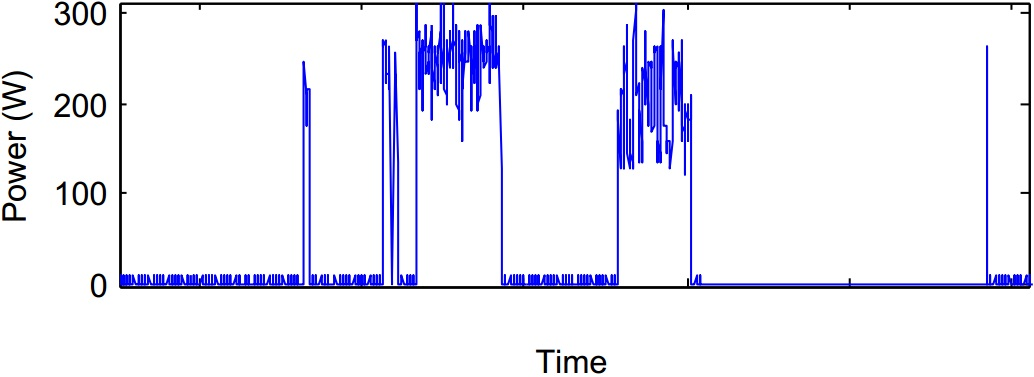
\includegraphics[scale=\exsca]{figures/EXpower.jpg}
   \caption{\smartsocket de la lampe}
  \end{minipage}
 \end{figure}
 \begin{figure}
  \centering
  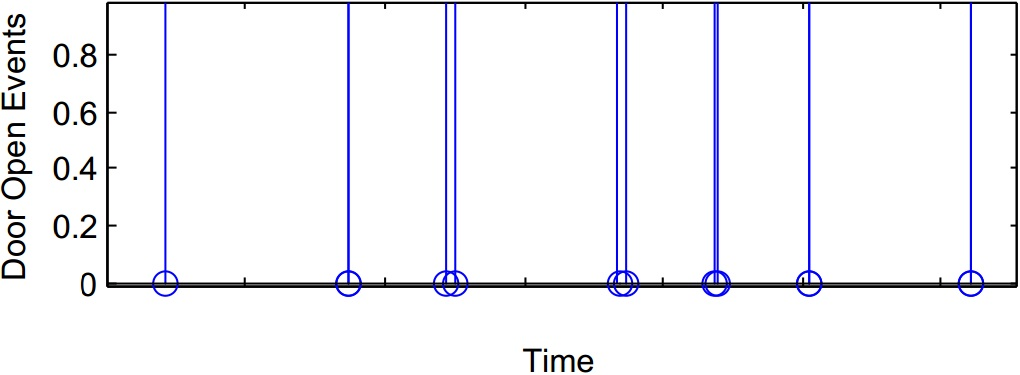
\includegraphics[scale=\exsca]{figures/EXdoor.jpg}
  \caption{Ouverture de la porte}
 \end{figure}
\end{frame}

\begin{frame}
 \frametitle{Résultats}
 Grâce à un algorithme qui baisse la température du chauffage lorsque la maison est innocupée, ils ont pu économiser 7,2\% d'énergie de chauffage.
 Le graphique suivant montre l'économie totale d'énergie par jour.
 \begin{figure}
  \centering
  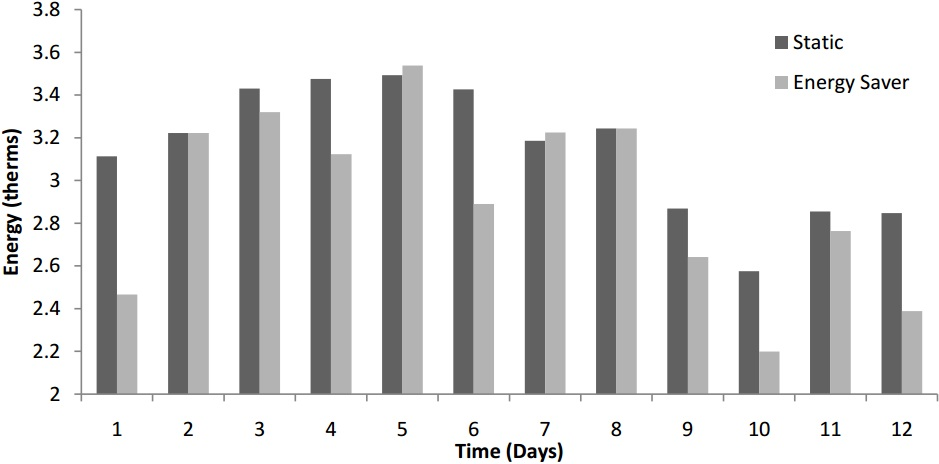
\includegraphics[scale=0.38]{figures/energysaver.jpg}
  \caption{Économie d'énergie totale}
 \end{figure} 
 Ils ont utilisé un algorithme se basant que sur l'occupation de la maison. Il existe de meilleurs algorithmes prenant en compte l'occupation de chaque pièces.
\end{frame}

 
 